% VoiceNotion - Chapitre I: Etude préalable
% Ce chapitre présente l'étude préliminaire du projet VoiceNotion



\section{Introduction}

Dans un monde où la productivité et l'efficacité sont devenues des priorités absolues, la prise de notes demeure un processus fondamental pour capturer et organiser l'information. Que ce soit pour les étudiants, les professionnels ou les créateurs de contenu, la capacité à saisir rapidement des idées, des concepts ou des informations est essentielle. Cependant, les méthodes traditionnelles de prise de notes présentent des limitations significatives, notamment en termes de vitesse, d'accessibilité et de flexibilité.

Cette étude préalable vise à explorer le contexte, les problématiques et les opportunités liés à la création d'une application de prise de notes pilotée par la voix, que nous avons nommée VoiceNotion. Notre analyse portera sur les défis actuels de la prise de notes, les solutions existantes sur le marché, et la manière dont notre approche innovante peut répondre aux besoins non satisfaits des utilisateurs.

\section{Problématiques}

La prise de notes traditionnelle, qu'elle soit manuscrite ou numérique, présente plusieurs défis majeurs que nous avons identifiés à travers notre recherche et nos observations:

\subsection{Limites de la saisie manuelle}

La saisie manuelle de notes, que ce soit à l'aide d'un stylo et papier ou d'un clavier, présente plusieurs inconvénients:

\begin{itemize}
    \item \textbf{Vitesse limitée:} La vitesse de frappe moyenne (40-60 mots par minute) ou d'écriture manuscrite (10-30 mots par minute) est souvent insuffisante pour capturer efficacement des informations lors de réunions, conférences ou sessions de brainstorming rapides.
    
    \item \textbf{Fatigue et inconfort:} La saisie prolongée peut entraîner une fatigue des mains et des poignets, particulièrement sur les appareils mobiles où les claviers virtuels offrent une expérience sous-optimale.
    
    \item \textbf{Attention divisée:} Le fait de devoir se concentrer sur la saisie divise l'attention de l'utilisateur, réduisant sa capacité à écouter activement ou à participer pleinement à une discussion.
\end{itemize}

\subsection{Accessibilité réduite}

Les méthodes traditionnelles de prise de notes présentent des obstacles d'accessibilité significatifs:

\begin{itemize}
    \item \textbf{Mobilité réduite:} Les personnes souffrant de limitations motrices peuvent éprouver des difficultés considérables avec la saisie manuelle.
    
    \item \textbf{Situations multi-tâches:} De nombreux contextes (conduite, marche, exercice) rendent la saisie manuelle difficile voire impossible.
    
    \item \textbf{Barrières linguistiques:} Pour les utilisateurs non natifs d'une langue, la saisie écrite peut présenter des difficultés supplémentaires par rapport à l'expression orale.
\end{itemize}

\subsection{Complexité de structuration}

L'organisation et la structuration efficaces des notes représentent un défi majeur:

\begin{itemize}
    \item \textbf{Effort post-capture:} La transformation de notes brutes en contenu structuré et organisé nécessite souvent un effort supplémentaire considérable.
    
    \item \textbf{Rigidité des formats:} De nombreuses applications de prise de notes offrent des structures rigides qui limitent la flexibilité et l'adaptabilité aux différents types de contenu.
    
    \item \textbf{Courbe d'apprentissage:} Les éditeurs avancés comme Notion requièrent un investissement initial en temps pour maîtriser leurs fonctionnalités.
\end{itemize}

% \begin{figure}[H]
%     \centering
%     \includegraphics[width=0.8\textwidth]{../assets/docs/note_taking_challenges.png}
%     \caption{Défis de la prise de notes traditionnelle}
%     \label{fig:note_taking_challenges}
% \end{figure}

\section{Solution et objectif}

Face à ces problématiques, VoiceNotion propose une approche novatrice qui combine la puissance de la reconnaissance vocale, de l'intelligence artificielle et d'un éditeur de notes par blocs inspiré de Notion. Notre solution vise à créer une expérience de prise de notes qui soit à la fois rapide, accessible et puissante.

\subsection{Concept de VoiceNotion}

VoiceNotion est une application mobile et web qui permet aux utilisateurs de créer, éditer et organiser des notes principalement à travers des commandes vocales. L'application transforme la voix en texte structuré et permet d'effectuer diverses actions d'édition sans nécessiter d'interactions manuelles complexes.

\begin{itemize}
    \item \textbf{Saisie vocale intelligente:} Utilisation de l'API Gemini pour une transcription précise et une compréhension contextuelle des commandes.
    
    \item \textbf{Éditeur par blocs:} Interface inspirée de Notion permettant une organisation flexible du contenu en blocs (texte, listes, tableaux, images, etc.).
    
    \item \textbf{Commandes vocales complètes:} Capacité à effectuer toutes les actions d'édition courantes (formatage, création de listes, ajout de blocs, navigation) par la voix.
    
    \item \textbf{Expérience mobile-first:} Conçue d'abord pour les appareils mobiles, avec une interface adaptée aux écrans tactiles et aux contextes d'utilisation en déplacement.
\end{itemize}

% \begin{figure}[H]
%     \centering
%     \includegraphics[width=0.7\textwidth]{../assets/docs/voicenotion_concept.png}
%     \caption{Concept de VoiceNotion: fusion entre commandes vocales et éditeur par blocs}
%     \label{fig:voicenotion_concept}
% \end{figure}

\subsection{Objectifs du projet}

Le développement de VoiceNotion vise à atteindre plusieurs objectifs clés:

\begin{itemize}
    \item \textbf{Accélérer la prise de notes:} Permettre une saisie jusqu'à 3 fois plus rapide qu'avec un clavier traditionnel.
    
    \item \textbf{Améliorer l'accessibilité:} Rendre la prise de notes accessible aux personnes à mobilité réduite et dans des contextes où la saisie manuelle est difficile.
    
    \item \textbf{Simplifier la structuration:} Faciliter l'organisation du contenu grâce à des commandes vocales intuitives pour la création et la manipulation de blocs.
    
    \item \textbf{Offrir une flexibilité maximale:} Supporter divers cas d'utilisation, des notes rapides aux documents structurés complexes.
    
    \item \textbf{Garantir une expérience utilisateur fluide:} Proposer une interface intuitive qui minimise la friction entre l'intention de l'utilisateur et sa réalisation.
\end{itemize}

\section{Avantages du projet}

\begin{figure}[H]
    \centering
    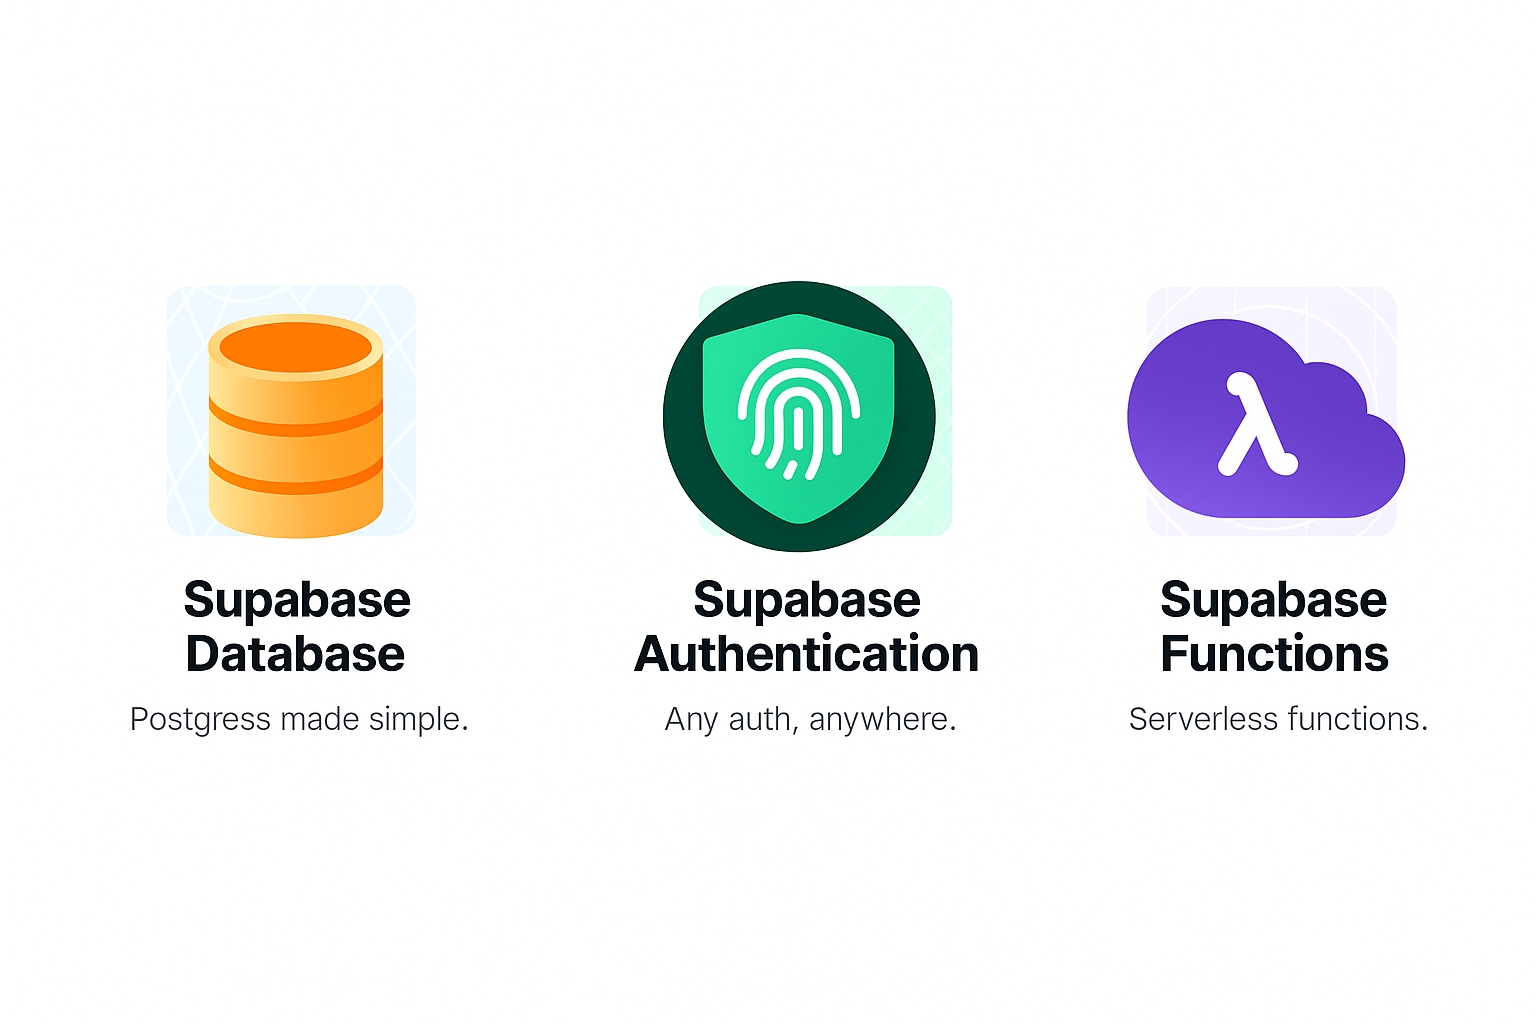
\includegraphics[width=\textwidth]{assets/docs/golobal-diagrams/supabase-feaature.png}
    \caption{Architecture des fonctionnalités principales de VoiceNotion grâce à Supabase. Cette vue globale illustre l'intégration des services backend, la gestion des données et la sécurité, offrant une base robuste à l'application.}
\end{figure}

VoiceNotion offre plusieurs avantages distincts par rapport aux solutions existantes sur le marché:

\subsection{Efficacité accrue}

\begin{itemize}
    \item \textbf{Vitesse de saisie supérieure:} La dictée vocale permet une saisie moyenne de 120-150 mots par minute, soit 2-3 fois plus rapide que la frappe.
    
    \item \textbf{Réduction du temps de formatage:} Les commandes vocales pour le formatage et la structuration éliminent le besoin de manipulations manuelles complexes.
    
    \item \textbf{Attention préservée:} Les utilisateurs peuvent se concentrer davantage sur le contenu et moins sur le processus de saisie.
\end{itemize}

\subsection{Accessibilité améliorée}

\begin{itemize}
    \item \textbf{Inclusion:} Solution accessible aux personnes à mobilité réduite ou souffrant de troubles musculosquelettiques.
    
    \item \textbf{Utilisation en contexte mobile:} Possibilité de prendre des notes en déplacement, pendant l'exercice ou dans d'autres situations où les mains sont occupées.
    
    \item \textbf{Réduction de la barrière linguistique:} Plus facile pour les utilisateurs non natifs qui s'expriment mieux oralement qu'à l'écrit.
\end{itemize}

\subsection{Flexibilité et puissance}

\begin{itemize}
    \item \textbf{Structure par blocs:} Organisation flexible du contenu adaptée à différents types de notes (cours, réunions, idées, projets).
    
    \item \textbf{Multimodalité:} Possibilité de basculer facilement entre saisie vocale et manuelle selon le contexte.
    
    \item \textbf{Adaptation contextuelle:} L'intelligence artificielle permet d'adapter l'interprétation des commandes au contexte spécifique de l'utilisateur.
\end{itemize}

% \begin{figure}[H]
%     \centering
%     \includegraphics[width=0.8\textwidth]{../assets/docs/voicenotion_advantages.png}
%     \caption{Avantages comparatifs de VoiceNotion}
%     \label{fig:voicenotion_advantages}
% \end{figure}

\section{Conclusion}

Cette étude préalable a permis d'identifier clairement les problématiques actuelles de la prise de notes traditionnelle et de poser les bases conceptuelles de VoiceNotion comme solution innovante. En combinant la puissance de la reconnaissance vocale, de l'intelligence artificielle et d'un éditeur par blocs flexible, VoiceNotion a le potentiel de transformer radicalement l'expérience de prise de notes pour un large éventail d'utilisateurs.

Le projet répond à des besoins réels et non satisfaits du marché, offrant une alternative plus rapide, plus accessible et plus flexible aux méthodes traditionnelles. Les chapitres suivants détailleront la planification, la conception et l'implémentation technique de cette solution, en mettant l'accent sur l'expérience utilisateur et la robustesse technique.

Dans un monde où l'information est abondante et le temps précieux, VoiceNotion vise à devenir un outil essentiel pour capturer, organiser et exploiter efficacement les idées et les connaissances. 